% !TeX root = main.tex

\section[A2: 3R Planar Robot]{3R Manipulator Kinematics and Workspace}

\subsection[A2.1: End effector position]{End effector tool position}

Assuming that the end effector is attached at $\mathbf{P_e}$ as shown in Figure \ref{fig:sfig-3r-given}, the state that describes the end effector is $(E_x, E_y, E_{\theta})$. The terms are described in Figure \ref{fig:3r-manipulator}. The end effector tool position is given by

\begin{equation}
    \begin{bmatrix}
    E_x \\ E_y \\ E_{\theta}
    \end{bmatrix} = \begin{bmatrix}
    a_x + b_x + c_x \\
    a_y + b_y + c_y \\
    \theta_1 + \theta_2 + \theta_3
    \end{bmatrix} = \begin{bmatrix}
    l_1 \cos(\theta_1) + l_2 \cos(\theta_1 + \theta_2) + l_3 \cos(\theta_1 + \theta_2 + \theta_3) \\
    l_1 \sin(\theta_1) + l_2 \sin(\theta_1 + \theta_2) + l_3 \sin(\theta_1 + \theta_2 + \theta_3) \\
    \theta_1 + \theta_2 + \theta_3
    \end{bmatrix}
\end{equation}

This is written in the following shorthand convention

\begin{equation}
    \begin{bmatrix}
    E_x \\ E_y \\ E_{\theta}
    \end{bmatrix} = \begin{bmatrix}
    l_1 c_1 + l_2 c_{12} + l_3 c_{123} \\
    l_1 s_1 + l_2 s_{12} + l_3 s_{123} \\
    \theta_1 + \theta_2 + \theta_3
    \end{bmatrix}
    \label{eq:3r-fk-equation}
\end{equation}

\begin{figure}[ht]
    \centering
    \begin{subfigure}[b]{0.3\textwidth}
        \centering
        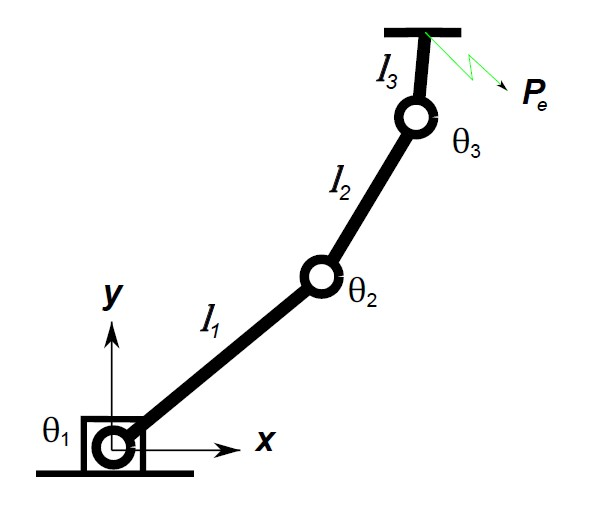
\includegraphics[width=\textwidth]{e2-3r-given.jpg}
        \caption{3R Robot}
        \label{fig:sfig-3r-given}
    \end{subfigure}
    \begin{subfigure}[b]{0.45\textwidth}
        \centering
        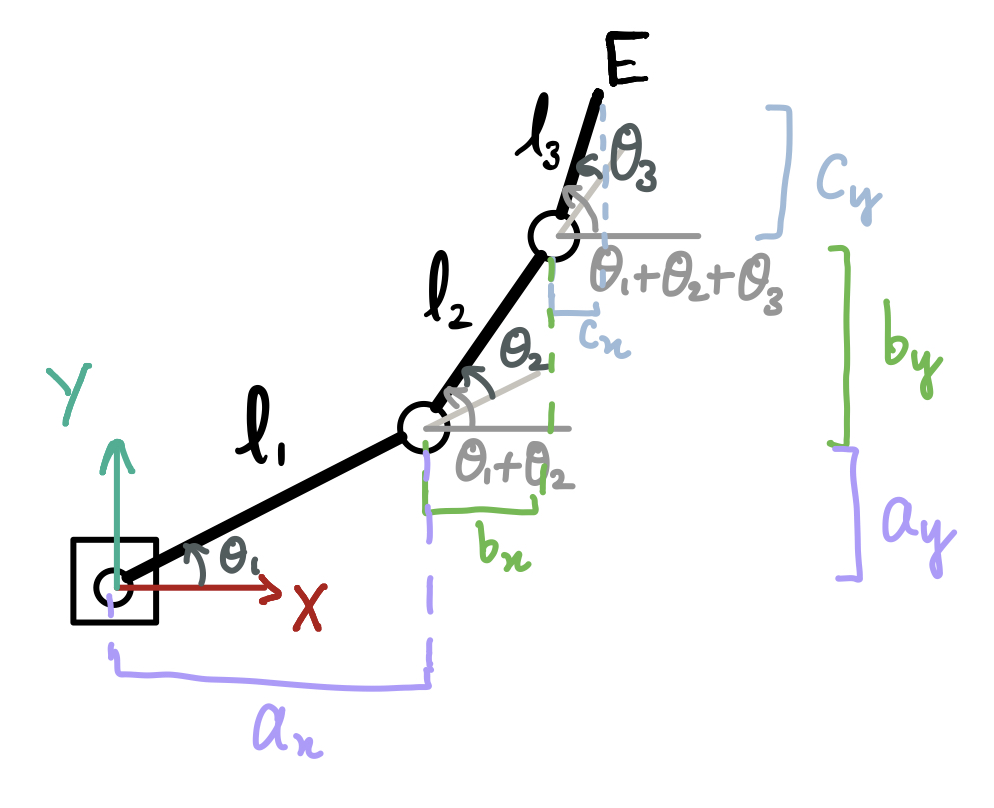
\includegraphics[width=\textwidth]{e2-3r-fk-graphics.PNG}        
        \caption{FK through geometry}
        \label{fig:sfig-3r-fk-geometry}
    \end{subfigure}
    \caption{3R robot and forward kinematics}
    \small
        In sub-figure \ref{sub@fig:sfig-3r-given}, the given manipulator is shown. 
        In sub-figure \ref{sub@fig:sfig-3r-fk-geometry}, the forward kinematics of the given 3R is depicted. Note that $a_x = l_1 \cos(\theta_1)$, $a_y = l_1 \sin(\theta_1)$, $b_x = l_2 \cos(\theta_1 + \theta_2)$, $b_y = l_2 \sin(\theta_1 + \theta_2)$, $c_x = l_3 \cos(\theta_1 + \theta_2 + \theta_3)$ and $c_y = l_3 \sin(\theta_1 + \theta_2 + \theta_3)$; these values can be derived from geometry. The end effector position, given as $\mathbf{P_e}$ in sub-figure \ref{sub@fig:sfig-3r-given} is written as $\mathbf{E} = (E_x, E_y, E_{\theta})$ in sub-figure \ref{sub@fig:sfig-3r-fk-geometry}.
    \label{fig:3r-manipulator}
\end{figure}

\subsection[A2.2: Workspace]{Forward Kinematics and Workspace}

The forward kinematics of the manipulator is given in Equation \ref{eq:3r-fk-equation}. However, to represent it as a homogeneous SE(2) transformation, we can write it as

\begin{equation}
    \begin{split}
        \mathbf{E} &= \begin{bmatrix}
            \cos(\theta_1 + \theta_2 + \theta_3) & -\sin(\theta_1 + \theta_2 + \theta_3) & l_1 \cos(\theta_1) + l_2 \cos(\theta_1 + \theta_2) + l_3 \cos(\theta_1 + \theta_2 + \theta_3) \\
            \sin(\theta_1 + \theta_2 + \theta_3) & \cos(\theta_1 + \theta_2 + \theta_3) & l_1 \sin(\theta_1) + l_2 \sin(\theta_1 + \theta_2) + l_3 \sin(\theta_1 + \theta_2 + \theta_3) \\
            0 & 0 & 1
            \end{bmatrix} \\
        &= \begin{bmatrix}
            c_{123} & -s_{123} & l_1 c_1 + l_2 c_{12} + l_3 c_{123} \\
            s_{123} & c_{123} & l_1 s_1 + l_2 s_{12} + l_3 s_{123} \\
            0 & 0 & 1
            \end{bmatrix}
    \end{split}
\end{equation}

The graphical derivation of this is shown in Figure \ref{fig:sfig-3r-fk-geometry} and has been derived earlier. This is implemented in code in Appendix \ref{app:a2.2-fk-code}. The code to generate Figure \ref{fig:3r-ws-dws} is implemented in Appendix \ref{app:a2.2-ws-dws-show-code}. The code for an interactive tool for demonstrating forward kinematics is in \ref{app:a2.2-3r-fk-interactive}.

\subsubsection*{Workspace}

\begin{enumerate}
    \item The \emph{reachable workspace} is given by the set of points that the manipulator can reach.
    \item The \emph{dexterous workspace} is given by the set of points that the manipulator can reach with any arbitrary orientation.
\end{enumerate}

These are shown in Figure \ref{fig:3r-ws-dws}, along with a few configurations. The reachable workspace is in the region bounded by black circles, the dexterous workspace is in the region bounded by \textcolor{red}{red circles}. The corresponding code is in Appendix \ref{app:a2.2-ws-dws-show-code}.

From figures \ref{fig:sfig-3r-dwso} and \ref{fig:sfig-3r-dwsi}, it is clear that whenever the \textcolor{magenta}{joint 2} can trace a full circle with radius $l_3$, the end effector (which will be at the center of that circle) will be in the dexterous workspace, as it will be possible to orient it at any angle at that endpoint.

\begin{figure}[!ht]
    \centering
    \begin{subfigure}[b]{0.45\textwidth}
        \centering
        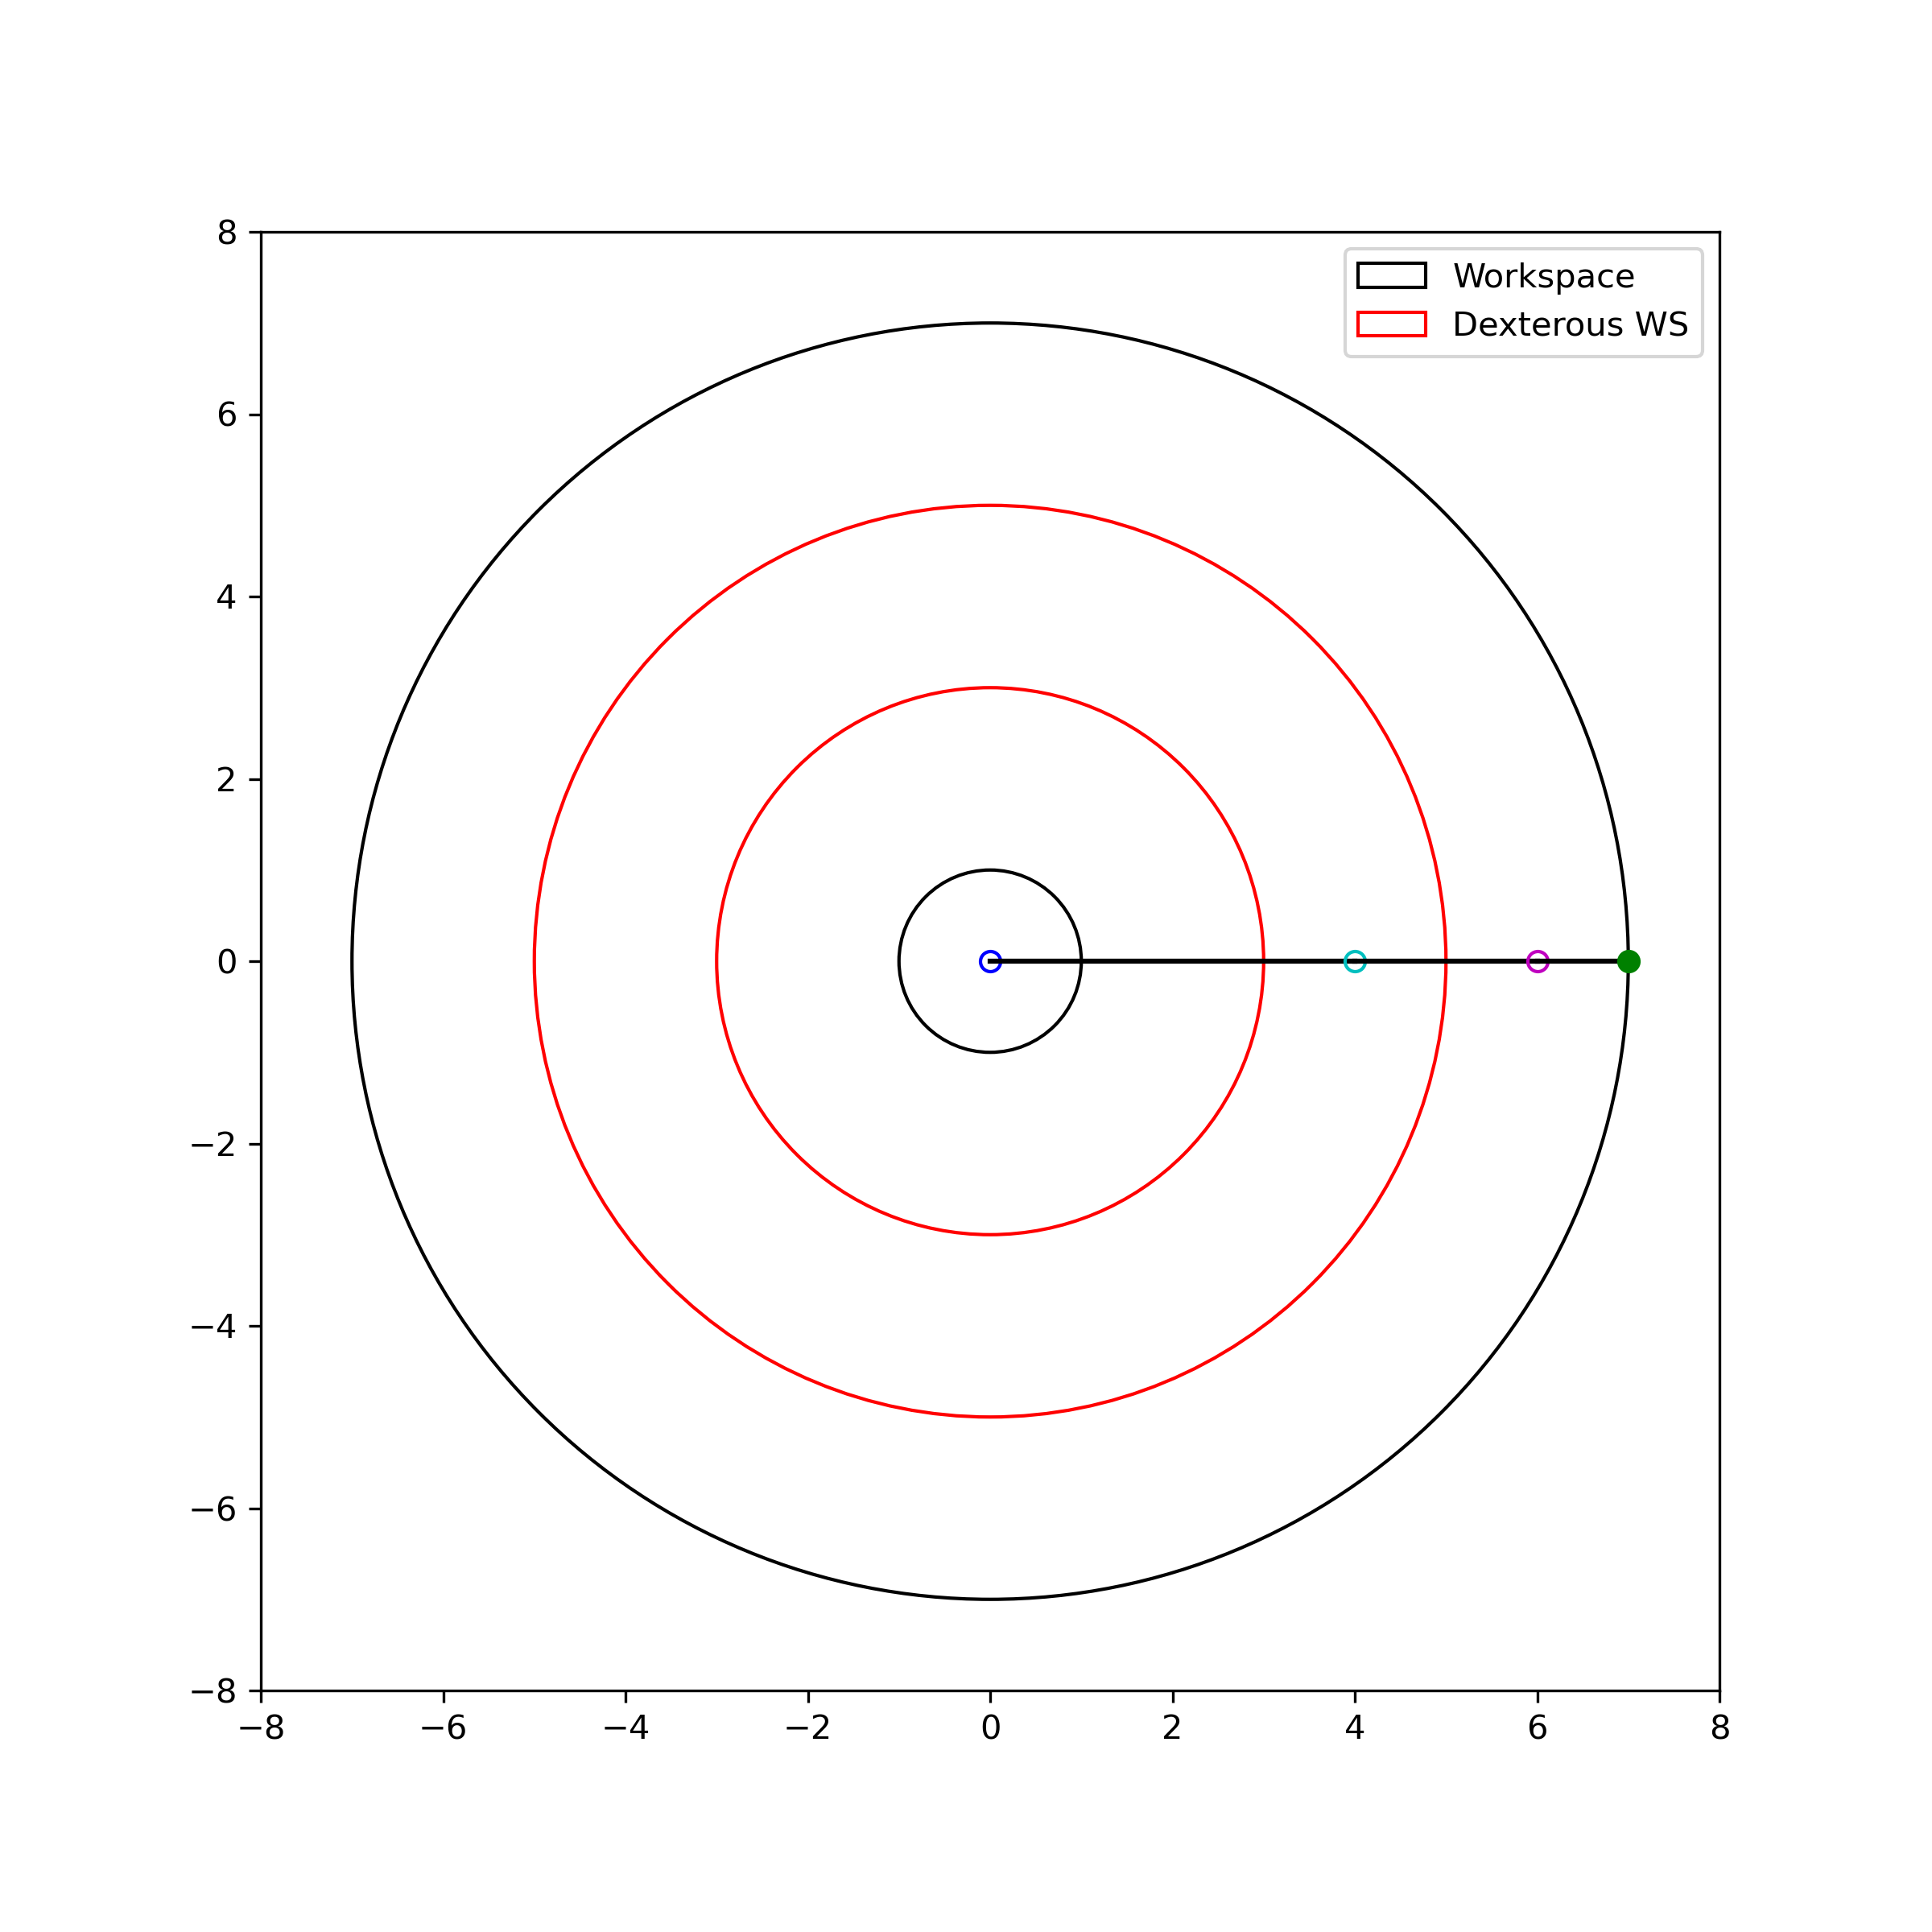
\includegraphics[width=\textwidth]{ex2-2-ws-outer.png}
        \caption{$(0, 0, 0)$}
        \label{fig:sfig-3r-wso}
    \end{subfigure}
    \begin{subfigure}[b]{0.45\textwidth}
        \centering
        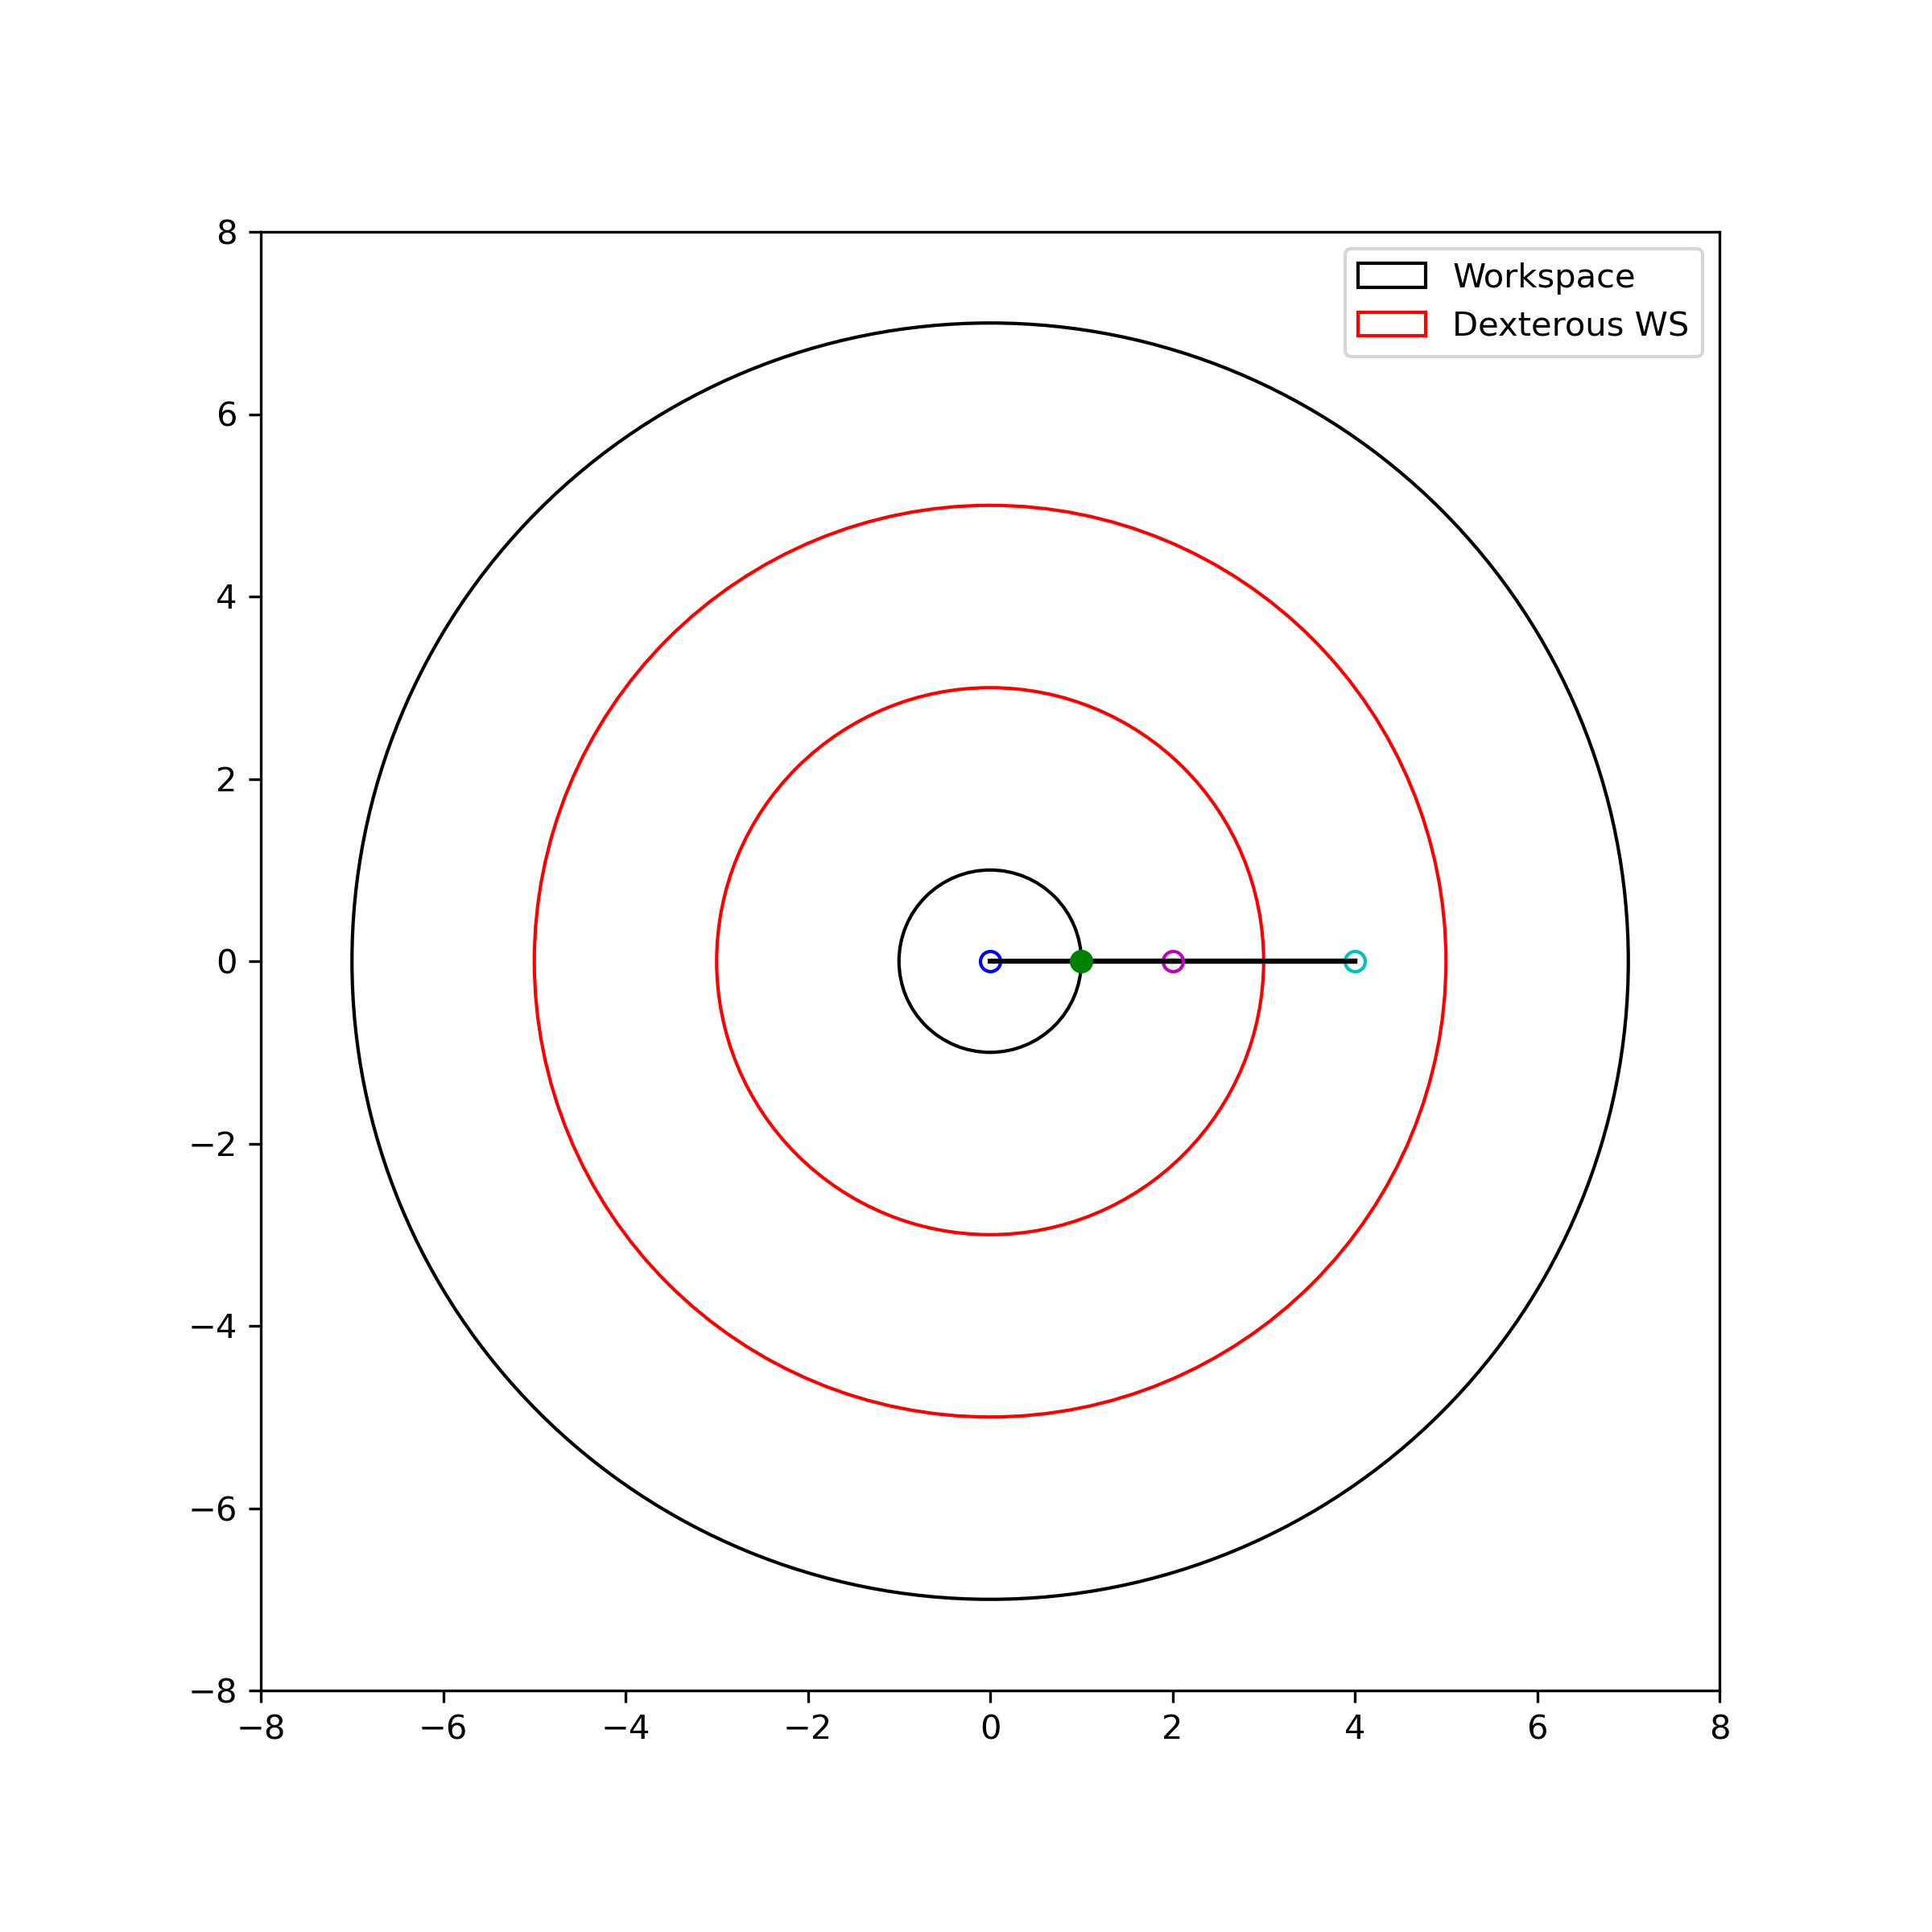
\includegraphics[width=\textwidth]{ex2-2-ws-inner.png}
        \caption{$(0, \pi, 0)$}
        \label{fig:sfig-3r-wsi}
    \end{subfigure}
    \begin{subfigure}[b]{0.45\textwidth}
        \centering
        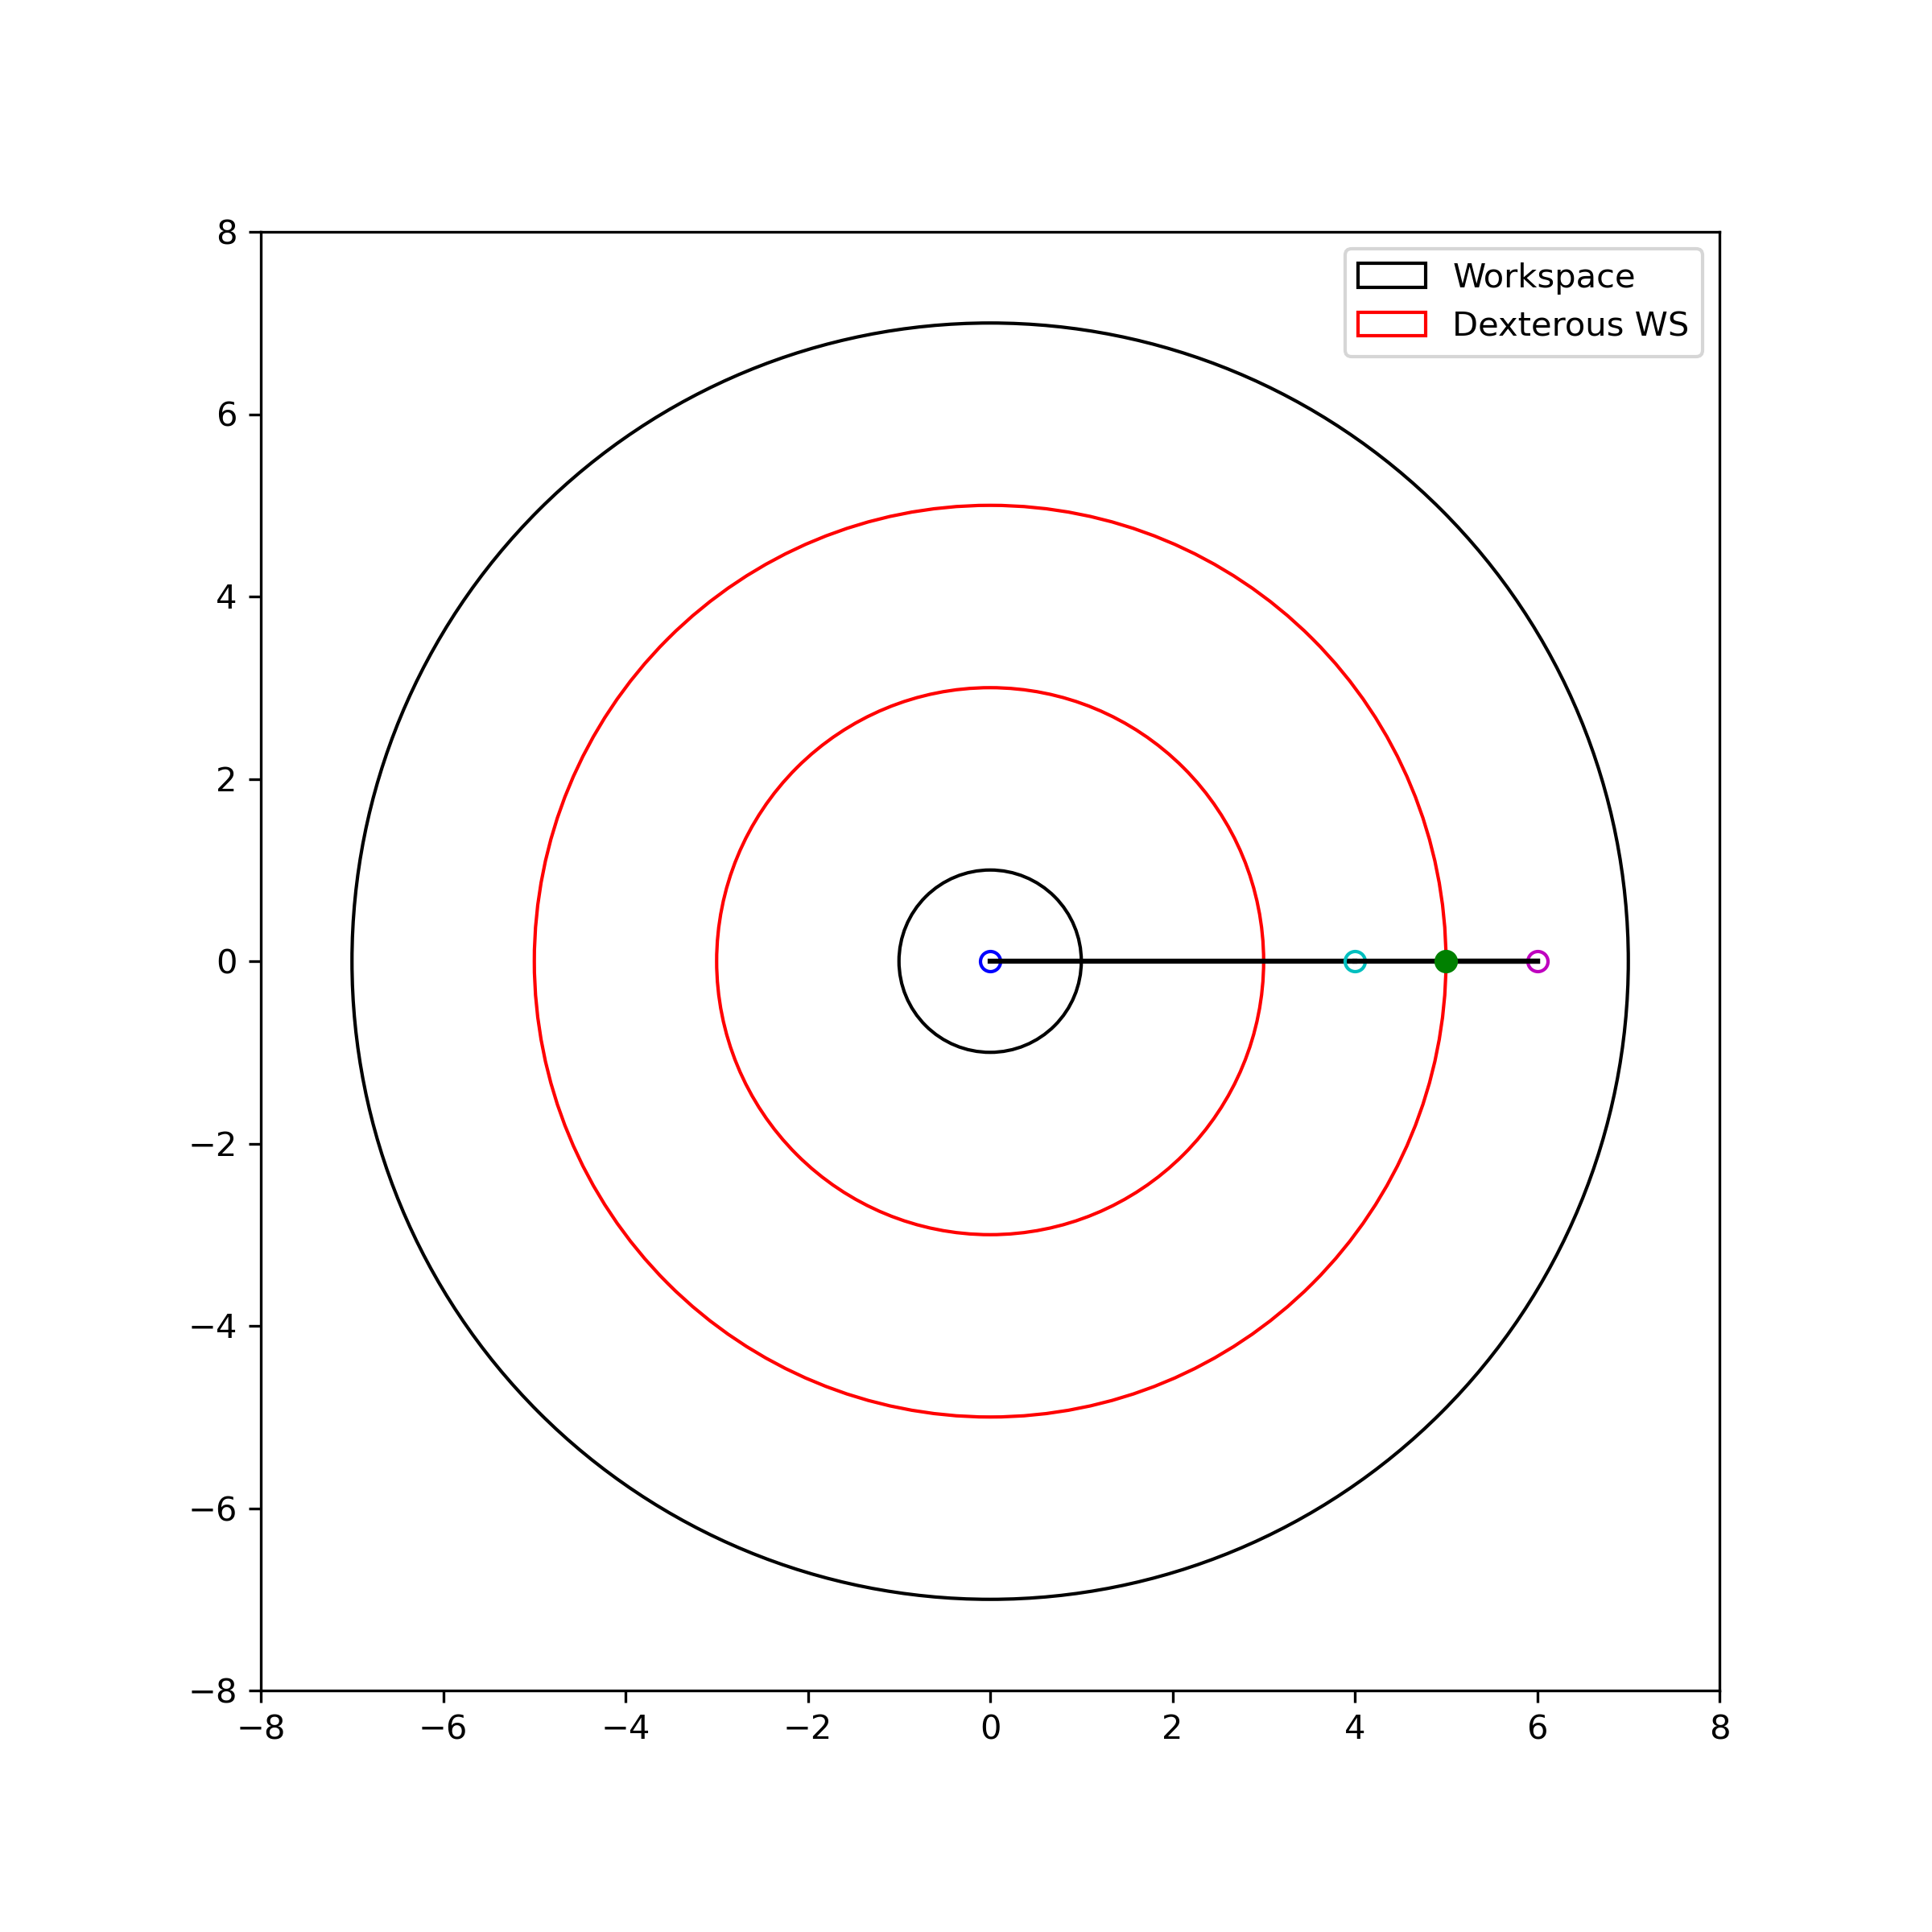
\includegraphics[width=\textwidth]{ex2-2-dws-outer.png}
        \caption{$(0, 0, \pi)$}
        \label{fig:sfig-3r-dwso}
    \end{subfigure}
    \begin{subfigure}[b]{0.45\textwidth}
        \centering
        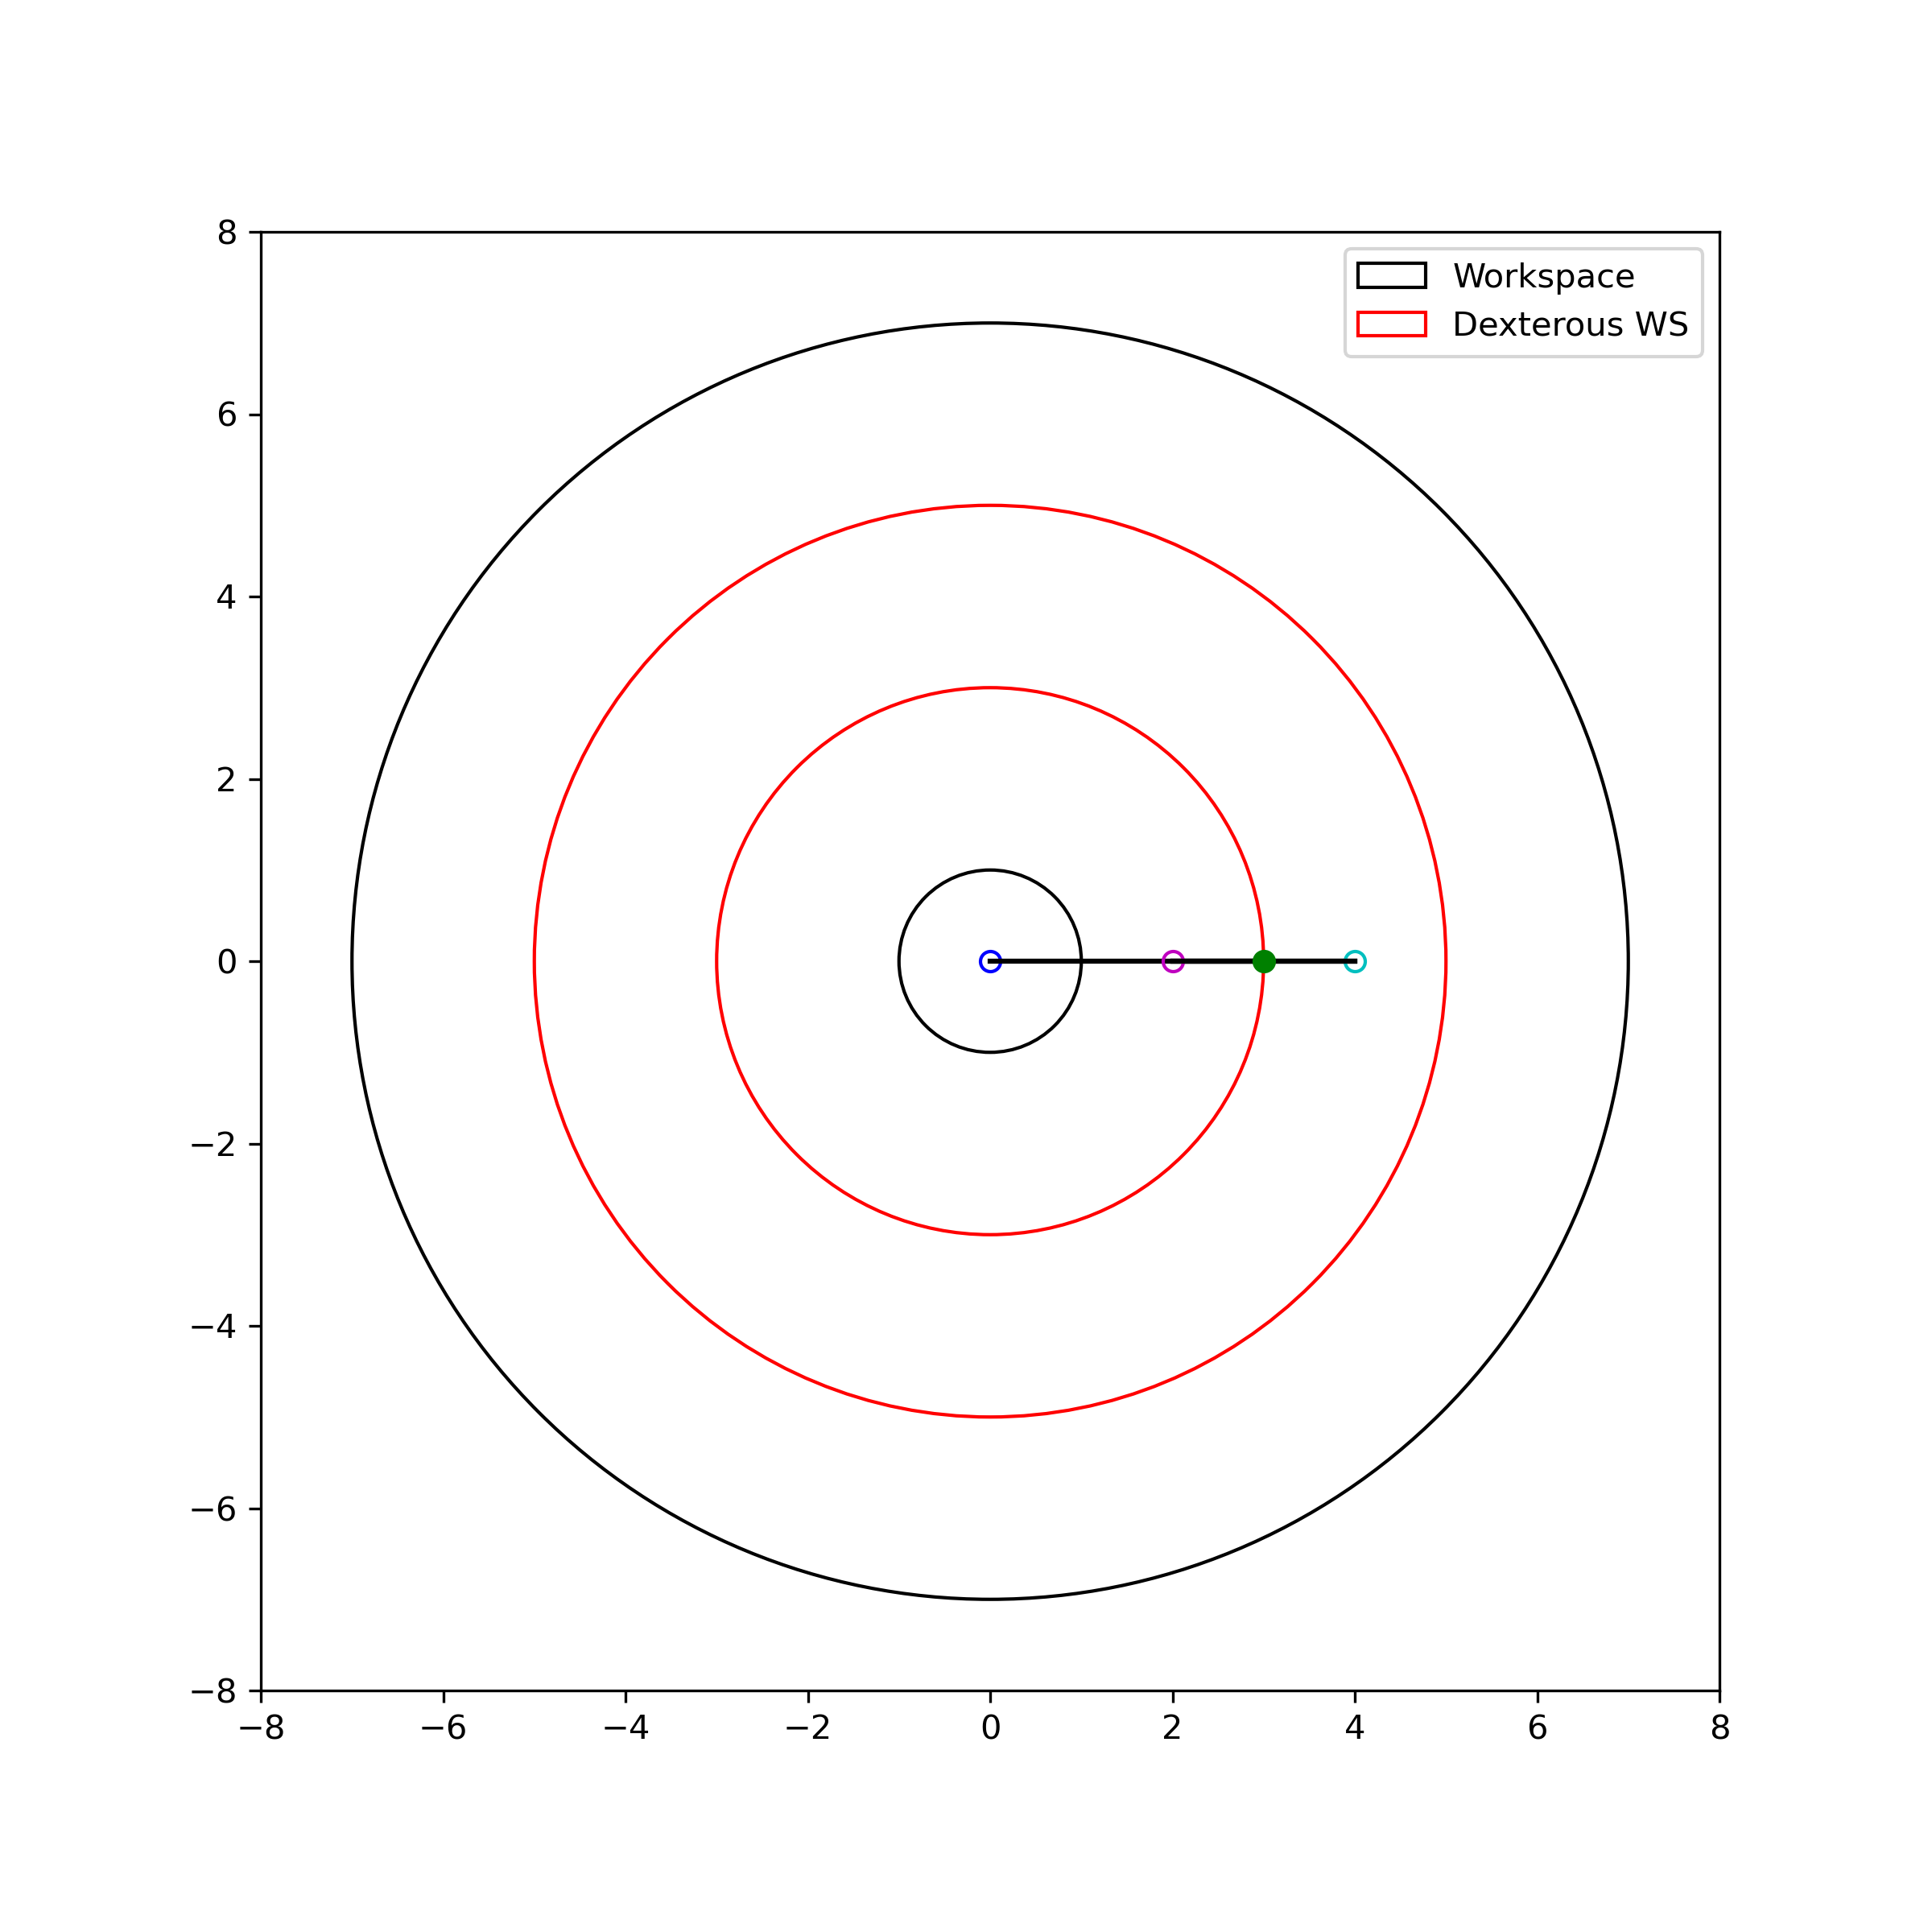
\includegraphics[width=\textwidth]{ex2-2-dws-inner.png}
        \caption{$(0, \pi, \pi)$}
        \label{fig:sfig-3r-dwsi}
    \end{subfigure}
    \caption{3R Workspace and Dexterous Workspace}
    \small
        The reachable workspace and the dexterous workspace of a 3R manipulator. For this figure, the link lengths are $l_1 = 1$, $l_2 = 2$, $l_3 = 4$. 
        The joint 1 is shown in \textcolor{blue}{blue circle}, the joint 2 is shown in \textcolor{cyan}{cyan circle}, the joint 3 is shown in \textcolor{magenta}{magenta circle} and the end effector is shown in \textcolor{Green}{green filled circle}. 
        The \textcolor{red}{red circles} show the bounds of the dexterous workspace and the black circles show the bounds of the reachable workspace. 
        The figures are captioned with the $(\theta_1, \theta_2, \theta_3)$ values for joint angles. 
        Sub-figures \ref{sub@fig:sfig-3r-wso} and \ref{sub@fig:sfig-3r-wsi} show the outer and inner limits of the \emph{reachable} workspace. Sub-figures \ref{sub@fig:sfig-3r-dwso} and \ref{sub@fig:sfig-3r-dwsi} show the outer and inner limits of the \emph{dexterous} workspace.
        The radius of outer black circle is $7$ unite, and the radius of inner black circle is $1$ unit. The radius of outer \textcolor{red}{red} circle is $5$ units and that of inner \textcolor{red}{red} circle is $3$ units.
        The corresponding code for this output can be found in Appendix \ref{app:a2.2-ws-dws-show-code} and \textbf{interactive code} is in Appendix \ref{app:a2.2-3r-fk-interactive}.
    \label{fig:3r-ws-dws}
\end{figure}
